\documentclass[a4paper]{article}
\usepackage[a4paper]{geometry}
\usepackage{amsmath}
\usepackage{amssymb}
\usepackage[utf8]{inputenc}
\usepackage{graphicx}
\usepackage{booktabs}
\usepackage[russian]{babel}
\usepackage{flafter}
\usepackage{caption}

\title{Лабораторная работа 2.1.6 \\Эффект Джоуля-Томсона}
\date{21 марта 2017 г.}
\author{Вячеслав Ждановский, студент 611 группы ФРКТ\\
Шамиль Вагабов, студент 611 группы ФРКТ\\
Станислав Токарев, студент 611 группы ФРКТ}
\begin{document}
	\pagenumbering{gobble}
	\maketitle
	\newpage
	\pagenumbering{arabic}
	\paragraph{Цель работы:} 1) определение изменения температуры углекислого газа пи протекании через малопроницаемую перегородк при разных начальных значениях давления и температуры; 2) вычисление по результатам опытов коэффициентов Ван-дер-Ваальса "a" и "b".
	\paragraph{В работе используются:} трубка с пористой перегородкой; труба Дьюара; термостат; термометры; дифференциальная теромпара; микровольтметр; балластный баллон; манометр.
	\section{Теория}
	Эффектом Джоуля-Томсона называется изменение температуры газа, медленно протекающего из области высокого в область низкого давления в условиях хорошей тепловой изоляции. В разреженных газах, которые приближаются по своим свойствам к реальному газу, при таком течении температура газа не меняется. Эффект Джоуля-Томсона демонстрирует отличие исследуемого газа от идеального.
	Рассмотрим стационарный поток газа между произвольными сечениями I и II трубки (до перегородки и после неё). 
	\begin{equation}
	A_1 - A_2 = \left(U_2 + \frac{\mu v^2_2}{2}\right) - \left(U_1 + \frac{\mu v^2_1}{2}\right)
	\end{equation}
	\begin{equation}
	H_1 - H_2 = (U_1 + P_1 V_1)-(U_2 + P_2 V_2)=\frac{1}{2}\mu (v^2_2-v^2_1)
	\end{equation}
	Выразим коэффициент Джоуля-Томсона для газа Ван-дер-Ваальса:
	\begin{equation}
	\mu_\text{д-т}=\frac{\Delta T}{\Delta P} \approx \frac{\frac{2a}{RT}-b}{C_p}
	\end{equation}
	Найдем связь между критической температуры и температуры инверсии, и зависимость температуры инверсии от параметров a, b: 
	\begin{equation}
	T_\text{инв}=\frac{27}{4}T_\text{кр}
	\end{equation}
	\begin{equation}
	T_\text{инв}=\frac{2a}{Rb}
	\end{equation}
		\newpage
	\section{Схема экспериментальной установки}
	\begin{figure}[ht!]
		\centering
		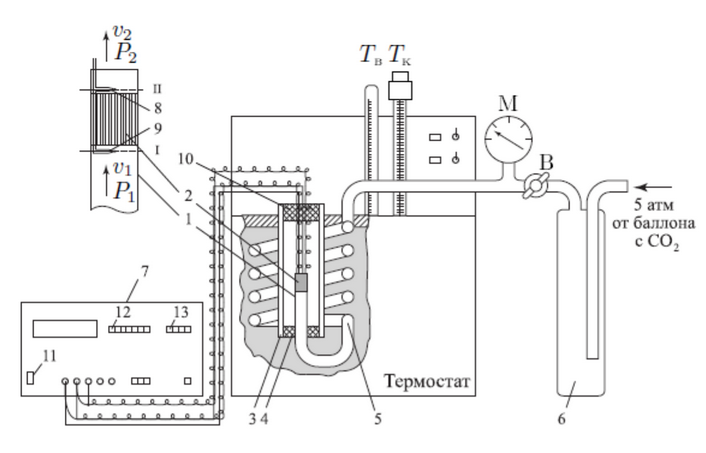
\includegraphics[height=80mm]{scheme.png}
		\caption{Схема экспериментальной установки \\ 1. Трубка, через которую пропускается исследуемый газ. \\ 2. Пористая перегородка. \\ 3. Труба Дьюара. \\ 4. Кольцо. \\ 5. Змеевик. \\ 6. Балластный баллон. \\ 7. Цифровой вольтметр. \\ 8 и 9. Спаи термопары. \\10. Пробка из пенопласта. \label{overflow}}
	\end{figure}
	\section{Ход работы}
	1. Включим термостат и устанавливаем комнатную температуру ${T_k}=23^o C$. \\
	2. Включим вольтметр и проведем измерения при различных $\Delta P$. Будем считать, что множитель термопары при ${T=T_k}$ равен $40.7$  $\frac{\text{мкВ}}{^o \text{C}}$. \\
	\begin{table}[h!]
 		\centering
	\begin{tabular}{|c|c|c|c|c|c|c|c|c|c|c|}
	\hline
U, мкв & 25	& -150 &	-135&	 -110&	-99&	-85&	-67&	-55&	-29 \\
\hline
$\Delta$T, $^o$C& 0,00	& -4,30	&-3,93	&-3,32	&-3,05	&-2,70 &	-2,26	& -1,97&	-1,33
 \\
\hline
$\Delta$P, атм& 0&	4&	3,7&	3&	2,7&	2,5&	2&	1,7&	1 \\
\hline
    	\end{tabular}
  		\caption{Измерения зависимости $\Delta$T от $\Delta$P в первом опыте}
	\end{table}
	3. Проведем измерения при T$=30$ $^o$C. Множитель термопары равен $41,6$ $\frac{\text{мкВ}}{^o \text{C}}$. \\
	\begin{table}[h!]
 		\centering
	\begin{tabular}{|c|c|c|c|c|c|c|c|}
	\hline
U, мкв & 40&	-138 &	-128	&-95	&-81&	-75	&-53
 \\
\hline
$\Delta$T, $^o$C& 0,00&	-4,28&	-4,04&	-3,25&	-2,91&	-2,76&	-2,24
  \\
\hline
$\Delta$P, атм& 0&	4&	3,7&	3&	2,7&	2,5	& 2\\
\hline
    	\end{tabular}
  		\caption{Измерения зависимости $\Delta$T от $\Delta$P во втором опыте	}
	\end{table}
	4. Проведем измерения при T$=40$ $^o$C. Множитель термопары равен $42,5$ $\frac{\text{мкВ}}{^o \text{C}}$. 
	\begin{table}[h!]
 		\centering
	\begin{tabular}{|c|c|c|c|c|c|}
	\hline
U, мкв & 6&	-126&	-81&	-44&	-15
 \\
\hline
$\Delta$T, $^o$C& 0,00	&-3,11&	-2,05&	-1,18&	-0,49

  \\
\hline
$\Delta$P, атм& 0&4&	3& 2 &1\\
\hline
    	\end{tabular}
  		\caption{Измерения зависимости $\Delta$T от $\Delta$P в третьем опыте	}
	\end{table}
	\begin{figure}[ht!]
		\centering
		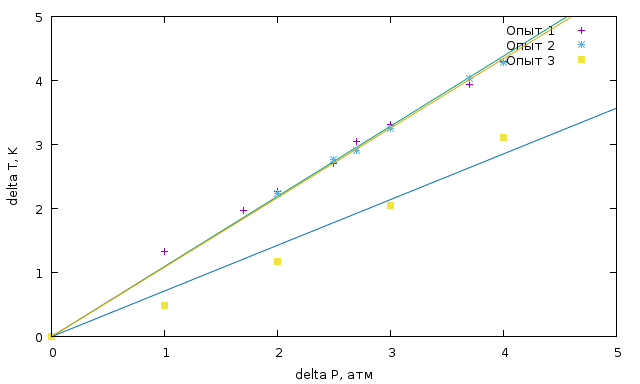
\includegraphics[width=125mm]{plot.png}
		\caption{Зависимости $\Delta$T от $\Delta$P\label{overflow}}
	\end{figure}
	5. Найдем из графиков коэффициенты Джоуля-Томсона: 
	\begin{table}[h!]
 		\centering
	\begin{tabular}{|c|c|c|c|}
	\hline
	T, $^o C$ & 23 & 30 & 40 \\
	\hline
	$\mu_\text{д-т}$ $\frac{^o C}{atm}$& 1.10 & 1.08 & 0.82 \\
	\hline
	$\sigma_\text{д-т (случ)}$ $\frac{^o C}{atm}$& 0.02 & 0.01 & 0.04 \\
	\hline
	$\sigma_\text{д-т}$ $\frac{^o C}{atm}$& 0.03 & 0.02 & 0.04 \\
	\hline
	\end{tabular}
  		\caption{Найденные коэффициенты Джоуля-Томсона}
	\end{table}
	6. Используя уравнение (3), найдем a и b.
	\begin{figure}[ht!]
		\centering
		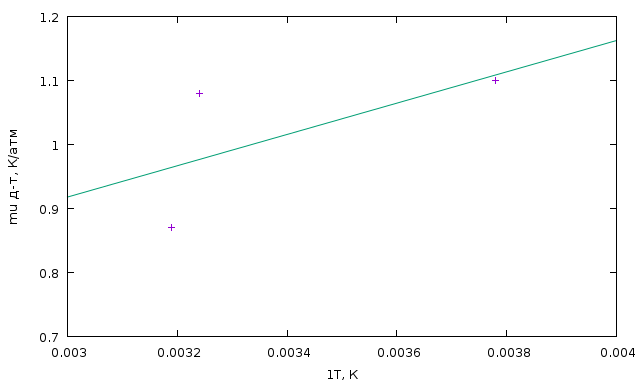
\includegraphics[width=125mm]{plot2.png}
		\caption{Зависимость коэффициента Джоуля-Томсона от температуры.\label{overflow}}
	\end{figure}
	Получаем $a=(64.7 \pm 24.6)\cdot 10^{-2}$ $\frac{\text{Дж}^2}{Па\cdot \text{моль}^2}$; $b=(14,0 \pm 7.0) \cdot 10^{-5} \frac{\text{Дж}}{K \cdot \text{моль}}$; $T_\text{инв}=(1,1 \pm 0.7) \cdot 10^3 K$
	\section{Контрольные вопросы}
	1. Во-первых, в реальном газе мы учитываем, что молекулы имеют конечные размеры. Иными словами, для второй молекулы некоторый объем является запрещенным из-за наличия первой молекулы. Во-вторых, мы учитываем, что молекулы притягиваются друг к другу. Одним из механизмов такого притяжения может быть перераспределение зарядов внутри молекул и образование диполей.\\
	2. Газ при достаточно большом , но постоянном давлении вынуждают протекать через теплоизолированную пористую перегородку. Это значит, что протекание газа происходит адиабатно. Сопротивление перегородки приводит к тому, что на ней теряется часть давления газа и газ выходит из перегородки при более низком давлении. Следовательно, газ расширяется(дросселируется). Для того чтобы течение газа было стационарным, т.е. происходило при постоянных значениях давлений по обе стороны дросселя( дроселем называют любое устройство, представляющее сопротивление для газа, в технических установках для охлаждения газов вместо пористой перегородки используется достаточно узкие сопла), необходим какой нибудь насос, который поддерживал бы постоянным давление. \begin{figure}[ht!]
		\centering
		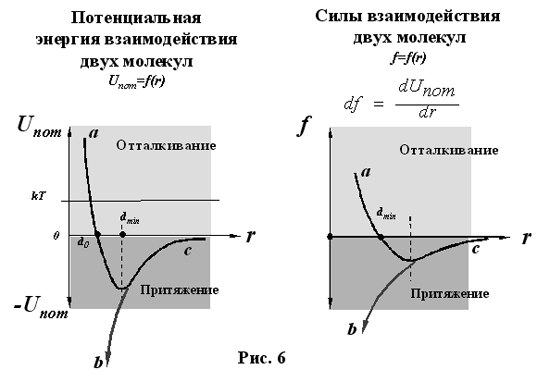
\includegraphics[width=75mm]{pic3.jpg}
		\caption{Кривые зависимости сил взаимодействия и взаимной потенциальной энергии двух молекул от расстояния между ними.\label{overflow}}
	\end{figure}\\
	3. Критическая температура - температура, выше которой газ не может быть превращен в жидкость ни при каком давлении. Температура инверсии - это температура при которой происходит изменение знака эффекта Джоуля - Томсона. $T_\text{инв} = \frac{2a}{Rb}$. При T < T\textsubscript{инв} $\Delta$T < 0 для тяжелых газов. При T > T\textsubscript{инв} $\Delta$T > 0: $H_2, He$ \\
	4. Из формулы (3) видно, что эффект Джоуля - Томсона для не очень плотного газа зависит от соотношения величин a и b, которые оказывают противоположное влияние на знак эффекта. Если силы взаимодействия между молекулами велики, так что превалирует "поправка на давление", то основную роль играет член, содержащий a, и $(\Delta T$/$\Delta P$) > 0, т.е. газ при расширении охлаждается. В обратном случае (малые a) ($\Delta T$/$\Delta P$) < 0 , т.е. газ нагревается. Идеальный газ отличается от реального тем, что в нём можно пренебречь потенциальной энергией взаимодействия молекул. Наличие этой энергии приводит к охлаждению или нагреванию реальных газов при расширении. При больших a потенциальная энергия молекул при их сближении уменьшается, а при удалении - при расширении газа - возрастает. Возрастание потенциальной энергии молекул происходит за счёт их кинетической энергии - температура газа при расширении падает. Аналогичные рассуждения позволяют понять, почему расширяющийся газ нагревается при больших b.
\end{document}